\documentclass{article}
\usepackage[utf8]{inputenc}
\usepackage{graphicx}	
\usepackage{longtable}
\usepackage{array}
\usepackage{pgfplots}
\pgfplotsset{compat = newest}

\title{Spadek swobodny}
\author{Bartosz Gruca}
\date{December 2022}

\begin{document}

\maketitle

\section{Wprowadzenie teoretyczne}

\begin{equation}
    h(t)=h_0- gt^2/2
\end{equation}

\section{Przebieg eksperymentu}

\begin{center}
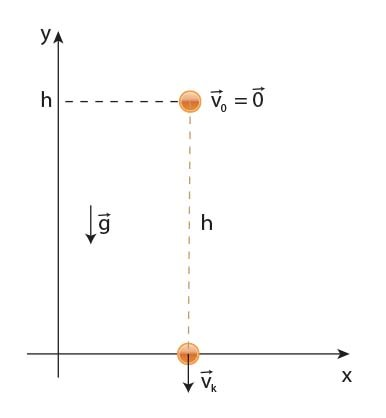
\includegraphics[scale=0.5]{zdj.jpg}
\end{center}

\section{Wyniki pomiaru}

\begin{center}
\begin{longtable}{|c|c|}
\caption{Czas i droga w spadku swobodnym} \\

\hline
t   & s(t)    \\ \hline 
0   & 0       \\ \hline
0,1 & 0,049   \\ \hline
0,2 & 0,196   \\ \hline
0,3 & 0,441   \\ \hline
0,4 & 0,784   \\ \hline
0,5 & 1,225   \\ \hline
0,6 & 1,764   \\ \hline
0,7 & 2,401   \\ \hline
0,8 & 3,136   \\ \hline
0,9 & 3,969   \\ \hline
1   & 4,9     \\ \hline
1,1 & 5,929   \\ \hline
1,2 & 7,056   \\ \hline
1,3 & 8,281   \\ \hline
1,4 & 9,604   \\ \hline
1,5 & 11,025  \\ \hline
1,6 & 12,544  \\ \hline
1,7 & 14,161  \\ \hline
1,8 & 15,876  \\ \hline
1,9 & 17,689  \\ \hline
2   & 19,6    \\ \hline
2,1 & 21,609  \\ \hline
2,2 & 23,716  \\ \hline
2,3 & 25,921  \\ \hline
2,4 & 28,224  \\ \hline
2,5 & 30,625  \\ \hline
2,6 & 33,124  \\ \hline
2,7 & 35,721  \\ \hline
2,8 & 38,416  \\ \hline
2,9 & 41,209  \\ \hline
3   & 44,1    \\ \hline
3,1 & 47,089  \\ \hline
3,2 & 50,176  \\ \hline
3,3 & 53,361  \\ \hline
3,4 & 56,644  \\ \hline
3,5 & 60,025  \\ \hline
3,6 & 63,504  \\ \hline
3,7 & 67,081  \\ \hline
3,8 & 70,756  \\ \hline
3,9 & 74,529  \\ \hline
4   & 78,4    \\ \hline
4,1 & 82,369  \\ \hline
4,2 & 86,436  \\ \hline
4,3 & 90,601  \\ \hline
4,4 & 94,864  \\ \hline
4,5 & 99,225  \\ \hline
4,6 & 103,684 \\ \hline
4,7 & 108,241 \\ \hline
4,8 & 112,896 \\ \hline
4,9 & 117,649 \\ \hline
5   & 122,5   \\ \hline
5,1 & 127,449 \\ \hline
5,2 & 132,496 \\ \hline
5,3 & 137,641 \\ \hline
5,4 & 142,884 \\ \hline
5,5 & 148,225 \\ \hline
5,6 & 153,664 \\ \hline
5,7 & 159,201 \\ \hline
5,8 & 164,836 \\ \hline
5,9 & 170,569 \\ \hline
6   & 176,4   \\ \hline
6,1 & 182,329 \\ \hline
6,2 & 188,356 \\ \hline
6,3 & 194,481 \\ \hline
6,4 & 200,704 \\ \hline
6,5 & 207,025 \\ \hline
6,6 & 213,444 \\ \hline
6,7 & 219,961 \\ \hline
6,8 & 226,576 \\ \hline
6,9 & 233,289 \\ \hline
7   & 240,1   \\ \hline
7,1 & 247,009 \\ \hline
7,2 & 254,016 \\ \hline
7,3 & 261,121 \\ \hline
7,4 & 268,324 \\ \hline
7,5 & 275,625 \\ \hline
7,6 & 283,024 \\ \hline
7,7 & 290,521 \\ \hline
7,8 & 298,116 \\ \hline
7,9 & 305,809 \\ \hline
8   & 313,6   \\ \hline
8,1 & 321,489 \\ \hline
8,2 & 329,476 \\ \hline
8,3 & 337,561 \\ \hline
8,4 & 345,744 \\ \hline
8,5 & 354,025 \\ \hline
8,6 & 362,404 \\ \hline
8,7 & 370,881 \\ \hline
8,8 & 379,456 \\ \hline
8,9 & 388,129 \\ \hline
9   & 396,9   \\ \hline
9,1 & 405,769 \\ \hline
9,2 & 414,736 \\ \hline
9,3 & 423,801 \\ \hline
9,4 & 432,964 \\ \hline
9,5 & 442,225 \\ \hline
9,6 & 451,584 \\ \hline
9,7 & 461,041 \\ \hline
9,8 & 470,596 \\ \hline
9,9 & 480,249 \\ \hline
10  & 490     \\ \hline
\end{longtable}
\end{center}


\section{Wnioski}
Lorem ipsum dolor sit amet, consectetur adipiscing elit. Proin congue sodales est a
dignissim. Maecenas interdum sagittis diam, nec tempus libero pellentesque quis. Curabitur
sagittis lectus at tortor consectetur lacinia sed ut nulla. Suspendisse ornare vehicula sagittis.
Cras sed molestie justo. Etiam eget dapibus nulla, eu pretium risus. In sed condimentum
massa. Praesent at varius erat. In vitae risus et massa eleifend tincidunt. Quisque feugiat
odio quis lacus sagittis pellentesque. Maecenas vel fermentum felis, sit amet convallis est.
 \\ 

\begin{center}
\begin{tikzpicture}
\begin{axis}[
    title={Droga i czas w spadku swobodnym},
    xlabel={T[s]},
    ylabel={S[m]},
    xmin=0, xmax=10,
    ymin=0, ymax=600,
    legend pos=north west,
    ymajorgrids=true,
    grid style=dashed,
]

\addplot+[
    only marks,
    scatter,
    mark=halfcircle*,
    mark size=1pt]
table[meta = s(t)]
{ScatterPlot.csv};

\addplot [
    domain=0:10, 
    samples=100, 
    color=red,
]
{(9.8*x*x)/2};

 
\end{axis}
\end{tikzpicture}
\end{center}

\end{document}
